\subsection{Resultados numéricos}

As Tabelas~\ref{tab:resultados-aleatorio}--\ref{tab:resultados-reverso}
apresentam média e desvio-padrão de cinco repetições por combinação. Para
$n>10\,000$, Insertion Sort e Selection Sort foram registrados como não
executados devido ao limite quadrático configurado; portanto, não são medições
nem estimativas.

\begin{table}[H]
\centering
\caption{Resultados para o cenário aleatório.}
\label{tab:resultados-aleatorio}
\footnotesize
\setlength{\tabcolsep}{3pt}
\begin{tabular}{lrrrr}
\toprule
Algoritmo & $n$ & Tempo médio $\pm$ DP (s) & Comparações & Movimentações \\
\midrule
Merge Sort & 10\,000 & 0.152693 $\pm$ 0.002502 & 120\,396 & 267\,232 \\
Quick Sort & 10\,000 & 0.168364 $\pm$ 0.009244 & 228\,277 & 234\,632 \\
Insertion Sort & 10\,000 & 18.784622 $\pm$ 1.253646 & 25\,107\,057 & 25\,107\,065 \\
Selection Sort & 10\,000 & 26.027759 $\pm$ 0.226308 & 49\,995\,000 & 19\,980 \\
Merge Sort & 100\,000 & 1.944215 $\pm$ 0.005681 & 1\,536\,336 & 3\,337\,856 \\
Quick Sort & 100\,000 & 2.053912 $\pm$ 0.006407 & 2\,867\,106 & 3\,034\,882 \\
Merge Sort & 1\,000\,000 & 37.055794 $\pm$ 2.819573 & 18\,673\,465 & 39\,902\,848 \\
Quick Sort & 1\,000\,000 & 40.909196 $\pm$ 3.829095 & 34\,127\,758 & 35\,509\,952 \\
\bottomrule
\end{tabular}
\end{table}

\begin{table}[H]
\centering
\caption{Resultados para o cenário ordenado.}
\label{tab:resultados-ordenado}
\footnotesize
\setlength{\tabcolsep}{3pt}
\begin{tabular}{lrrrr}
\toprule
Algoritmo & $n$ & Tempo médio $\pm$ DP (s) & Comparações & Movimentações \\
\midrule
Merge Sort & 10\,000 & 0.117302 $\pm$ 0.002478 & 64\,608 & 267\,232 \\
Quick Sort & 10\,000 & 0.700070 $\pm$ 0.008547 & 1\,129\,833 & 1\,088\,864 \\
Insertion Sort & 10\,000 & 0.010061 $\pm$ 0.000533 & 9\,999 & 9\,999 \\
Selection Sort & 10\,000 & 24.772758 $\pm$ 0.410491 & 49\,995\,000 & 0 \\
Merge Sort & 100\,000 & 1.473061 $\pm$ 0.010912 & 815\,024 & 3\,337\,856 \\
Quick Sort & 100\,000 & 37.251308 $\pm$ 12.871917 & 34\,247\,248 & 33\,839\,404 \\
Merge Sort & 1\,000\,000 & 32.856000 $\pm$ 2.913875 & 9\,884\,992 & 39\,902\,848 \\
Quick Sort & 1\,000\,000 & 771.234651 $\pm$ 70.408577 & 1\,058\,668\,552 & 1\,054\,611\,248 \\
\bottomrule
\end{tabular}
\end{table}

\begin{table}[H]
\centering
\caption{Resultados para o cenário reverso.}
\label{tab:resultados-reverso}
\footnotesize
\setlength{\tabcolsep}{3pt}
\begin{tabular}{lrrrr}
\toprule
Algoritmo & $n$ & Tempo médio $\pm$ DP (s) & Comparações & Movimentações \\
\midrule
Merge Sort & 10\,000 & 0.120620 $\pm$ 0.002175 & 69\,008 & 267\,232 \\
Quick Sort & 10\,000 & 0.490494 $\pm$ 0.001721 & 828\,748 & 782\,856 \\
Insertion Sort & 10\,000 & 35.747193 $\pm$ 0.639332 & 49\,995\,000 & 50\,004\,999 \\
Selection Sort & 10\,000 & 22.898518 $\pm$ 0.081678 & 49\,995\,000 & 10\,000 \\
Merge Sort & 100\,000 & 2.617466 $\pm$ 0.668734 & 853\,904 & 3\,337\,856 \\
Quick Sort & 100\,000 & 26.543369 $\pm$ 2.156796 & 24\,612\,475 & 24\,154\,004 \\
Merge Sort & 1\,000\,000 & 18.712902 $\pm$ 0.108989 & 10\,066\,432 & 39\,902\,848 \\
Quick Sort & 1\,000\,000 & 521.748054 $\pm$ 11.043940 & 754\,146\,232 & 749\,584\,436 \\
\bottomrule
\end{tabular}
\end{table}

\subsection{Gráfico de tempo}

A Figura~\ref{fig:tempo} apresenta somente execuções com status
\texttt{medido}; os casos inviáveis permanecem documentados nas tabelas. A
escala vertical é logarítmica para permitir a comparação entre tempos de ordens
de grandeza distintas.

\begin{figure}[H]
\centering
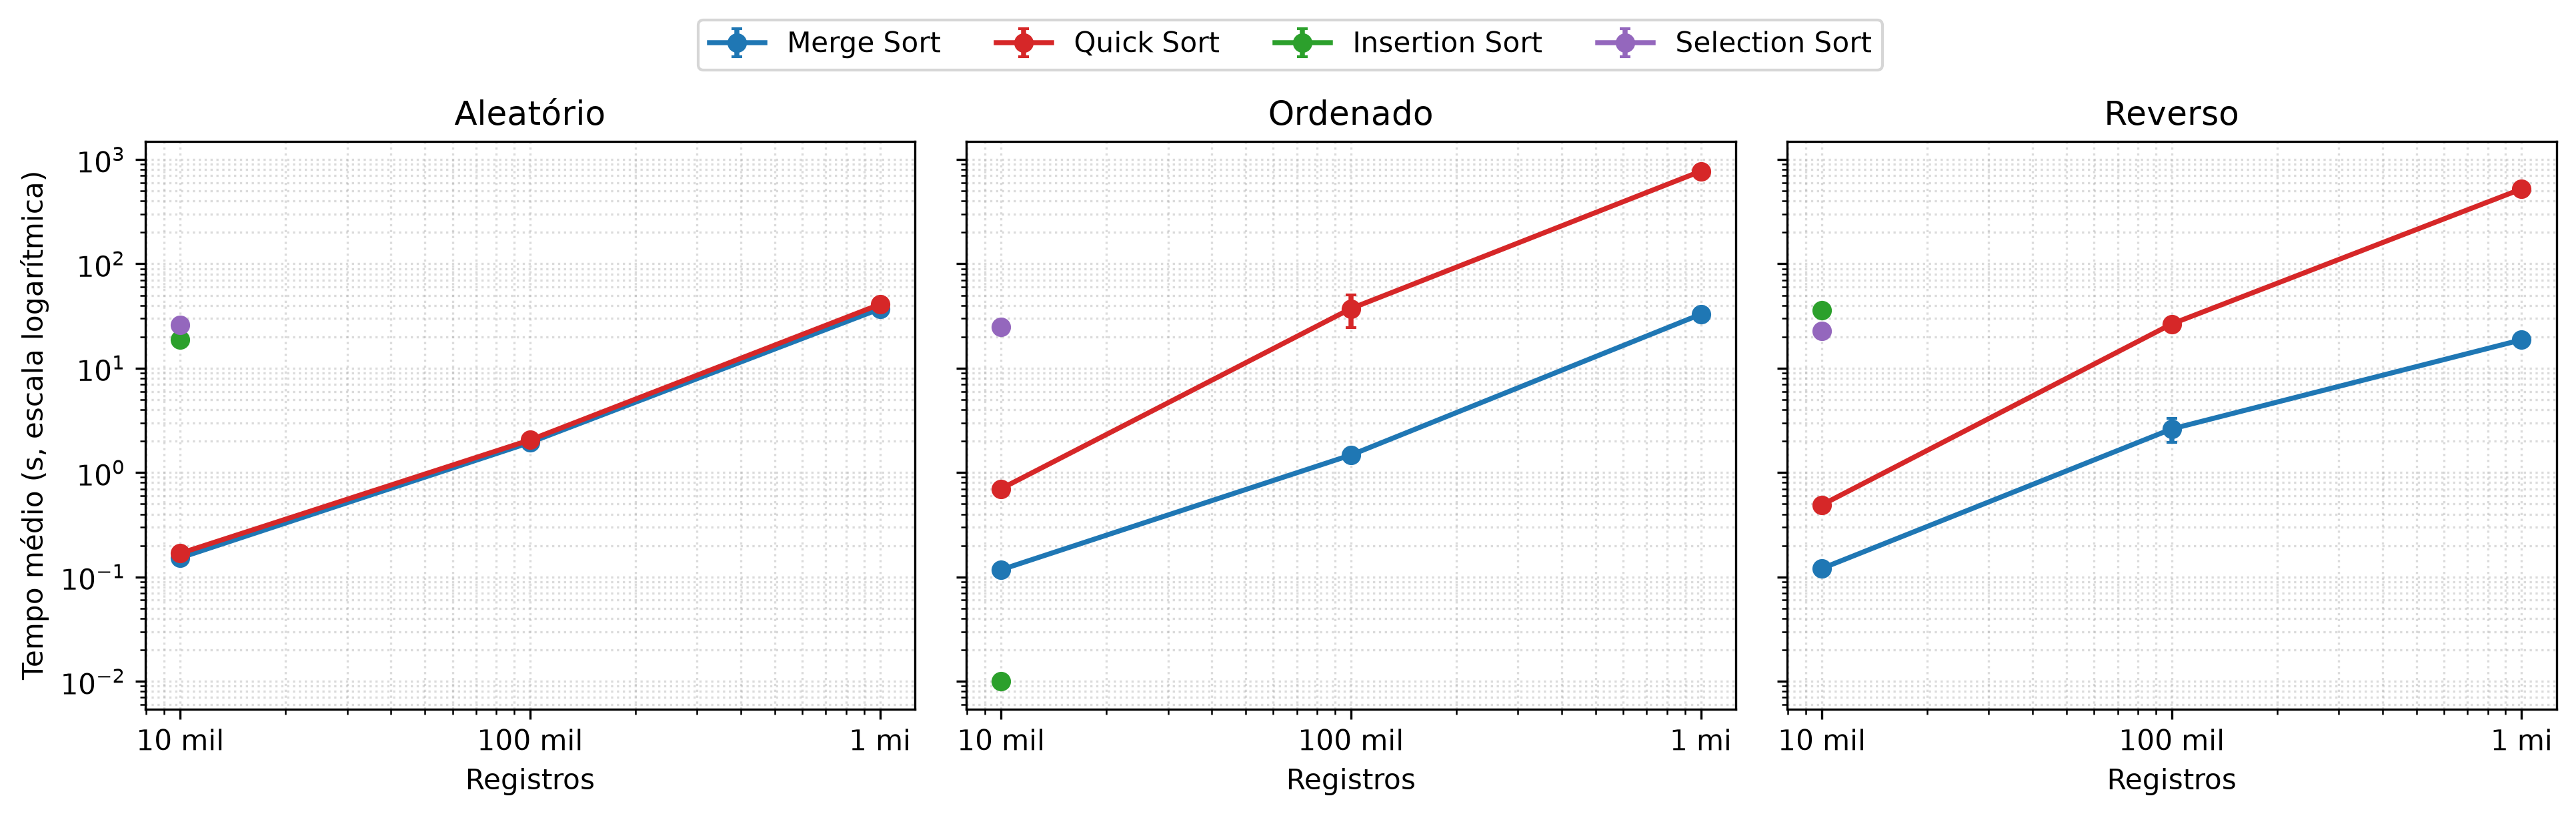
\includegraphics[width=\textwidth]{tempo_por_cenario.png}
\caption{Tempo médio de execução por algoritmo, tamanho e cenário. As barras
representam o desvio-padrão de cinco repetições; o eixo vertical usa escala
logarítmica.}
\label{fig:tempo}
\end{figure}
